\section{Історія розвитку методики}
\subsection{Перший досвід}
Мініінвазивні втручання радикально змінили хірургічну практику за останні три десятиріччя. Їх поява призвела до суттєвого покращення результатів за рахунок зменшення частоти післяопераційних ускладненнь, тривалості госпіталізації та співвідношення вартості до еффективності лікування.  Ці зміни торкнулись багатьох хірургічних спеціальностей, включаючи колоректальну хірургію, урологію, гінекологію та торокальну хірургію. Природньо, що зацікавленість хірургів в лапароскопічному доступі швидко розповсюдилась на гепатобіліарні втручання, спроби виконання яких в лапароскопічному варіанті було розпочато в 1987 році із першої лапароскопічної холецистектомії \cite{Litynski}. 

Для лікування уражень печінки лапароскопія була вперше впроваджена на початку 90х. На відміну від інших галузей, в печінковій хірургії лапароскопія зіткнулась із багатьма технічними перешкодами, пов'язаними із складною внутрішньою будовою та вразливою, схильною до кровотеч паренхімою печінки. Проте переваги лапароскопічного доступу, такі як покращена візуалізація, та зменшення післяопераційних ускладненнь, надали стимул для розвитку лапароскопічних резекцій печінки та здолання цих перешкод (\acrshort{llr}). 

Перші резекції печінки в лапароскопічному варіанті були виконані в 1991 році Reich H. \cite{Reich1991a} та  в 1992 Katkhouda N. \cite{Katkhouda1992} та Gagner M. \cite{GAGNER1992}. Ці операції були крайовими резекціями невеликих, переважно доброякісних, новоутворень. Невдовзі стало зрозуміло, що результати лапароскопічних операцій порівняні із традиційними відкритими втручаннями а \acrshort{llr} є безпечним та ефективним методом лікування. Відтоді \acrshort{llr} стала потенційною альтернативою відкритій резекції печінки (\acrshort{olr}). 

На початковому етапі розвиток методики був повільним, і наступні декілька років після першої згадки про \acrshort{llr} публікації містили лише опис поодиноких випадків атипових резекцій \cite{Klotz1993, Cunningham1995}. Перша анатомічна лапароскопічна лівобічна латеральна секцієектомія(\acrshort{llls}) виконана в 1996 році \cite{Azagra1996}  відновила інтерес до \acrshort{llr}  \cite{Hashizume1995}.  Із накопиченням досвіду покази до \acrshort{llr} були розширені до гемігепатектомій, складних сегментектомій, трисекцієектомій та навіть донорських резекцій при трансплантації печінки від живого донора \cite{Dagher2009, Cherqui2002, Jia2018}. 

\subsection{Погоджувальні конференції}

Від моменту виконання першої \acrshort{llr} кількість публікацій присвячених темі щорічно прогресивно збільшується (Рис. \ref{fig:PubMed_publications}). Стимулом до цього є посітйне вдосконалення ендохірургічного обладнання та хірургічної техніки.

Набутий досвід створив необхідність оцінки хірургічною спільнотою безпеки, відтворюваності та онкологічної ефективності \acrshort{llr}. Для вирішення цих завданнь та створення клінічних рекомендацій стосовно застосування \acrshort{llr} було  проведено декілька погоджувальних конференцій, висновки яких відображують процес становлення лапароскопічного методу та зміну відношення до нього хірургічного загалу. 

\begin{figure}[h]
\caption{Динаміка кількості публікацій в PubMed по запиту "laparosopic liver resection" по роках \cite{Hashizume1995}}
\centering
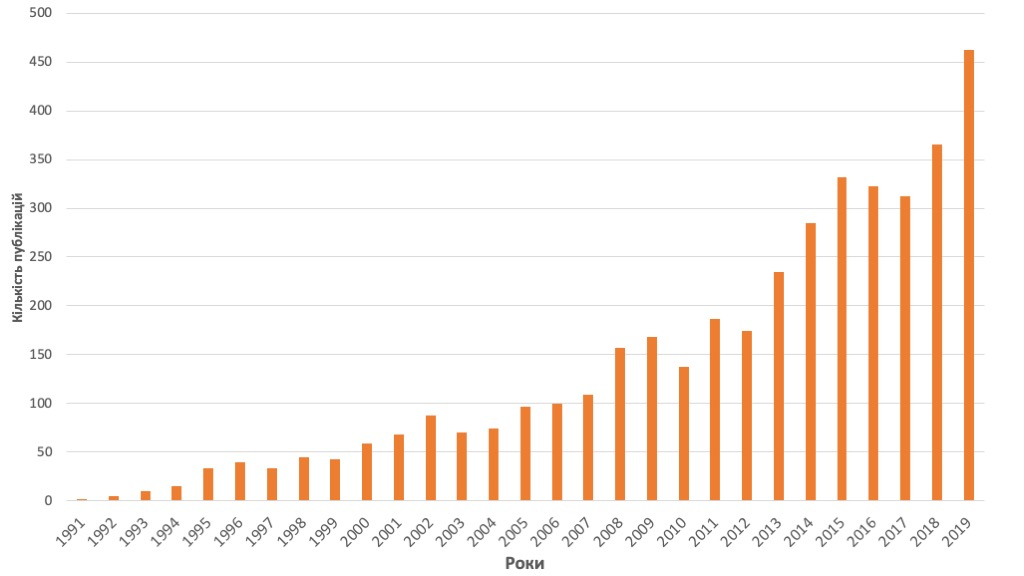
\includegraphics[width=0.9\textwidth]{Illustrations/Chapter_01/PubMed_publications.jpg}
\label{fig:PubMed_publications}
\end{figure}

\subsubsection{Перша погоджувальна конференція} 

Перша погоджувальна конференція відбулась в Луізвілі в листопаді 2008 року за участі 45 міжнародних експертів з гепатобіліарної хірургії. \cite{Buell2009}. За результатами обговорення до  \acrshort{llr} були віднесені чисто лапароскопічні, хенд-асистовані резекції печінки (\acrshort{hals}) та гибридні резекції печінки (\acrshort{hlr}) при яких початкова диссекція проводиться в лапароскопічному варіанті а розсічення паренхіми через мінілапаротомію. 

Прийнятними для видалення за допомогою \acrshort{llr} були визначені утворення, розміром менше 5 см, що розташовані в 2 - 6 сегментах печінки, а \acrshort{llls} було рекомендовано розглядати в якості стандартної практики. Також була показана принципова технічна можливість видалення новоутворень, локалізованих в будь яких сегментах печінки в лапароскопічному варіанті, проте обширні резекції печінки було рекомендовано зарезервувати за спеціалізованими гепатобіліарними центрами з великим досвідом як лапароскопічних втручаннь, так і резекційної хірургії печінки. 

Конверсію рекомендовано розглядати скоріше як необхідний крок для безпечного завершення складного втручання, ніж як ускладнення. Перед ургентною конверсією з приводу кровотечі хірург повинен докласти максимальних зусиль до зупинки кровотечі лапароскопічними методами. 

Вперше була показана можливість виконання донорського забору печінки при трансплантації від живого донора у дітей в лапароскопічному варіанті. Донорську \acrshort{llls} було оцінено, як експериментальну методику, що має великий потенціал але потребує детального вивчення. 

Загалом консенсус визначив \acrshort{llr} як безпечну альтернативу традиційним резекціям та рекомендував методику до подальшого вивчення та більш широкого впровадження досвідченими гепатобіліарними хірургами.

\subsubsection{Друга погоджувальна конференція} 

Друга погоджувальна конференція, яка відбулась в японському місті Моріока в жовтні 2014 році \cite{Kaneko2015}, була побудована за Цюріхсько-Датською моделлю, та включала в себе експертну панель з 43 досвідчених хірургів та 9 членів жюрі з 18 країн які оцінювали результати \acrshort{llr}. Для оцінки були запропоновані 17 запитаннь в категоріях переваги, ризики та технічні аспекти \acrshort{llr}. Доказова якість рекомендацій була оцінена за шкалою GRADE а ступінь розробки втручаннь за системою IDEAL \cite{Guyatt2008, McCulloch2009}. 

До малих резекцій (Minor resection) було віднести резекції 2 та меньше сегментів а до великих або обширних (Major resection) 3 та більше сегментів. Зважаючи на те, що технічна складність \acrshort{llls} та правобічної задньої або передньої секцієектомії в лапароскопічному варіанті значно відрізняються, резекції, до складу яких входять сегменти 7 або 8 було віднесено до технічно великих. 

За висновками експертного жюрі як малі так і великі \acrshort{llr} не гірші за відкриті в показниках операційної летальності, післяопераційних ускладненнь, чистоті резекційного краю, загальної виживаності, вартості операції та мають перевагу в більш короткому терміні перебування в стаціонарі, меншій крововтраті. Експерти погодились з тим, що результати лапароскопічних донорських заборів не відрізнялись від відкритих у високоспеціалізованих центрах. У якості додаткового висновку жюрі зазначило, що великі \acrshort{llr} вимагають високого рівню хірургічних навичок та тривалої кривої навчання.

Основними досягненнями конференції було по-перше визнання того, що  \acrshort{llr} за більшістю показників не поступаються, а за окремими показниками перевершують відкриті втручання, а по-друге рекомендація використовувати малі \acrshort{llr} в якості стандарту надання допомоги.

\subsubsection{Третя погоджувальна конференція та створення клінічних рекомендацій} 

Подальший еспотенціальний ріст кількості \acrshort{llr} призвів до того, що в лютому 2017 року в Саузхемптоні була проведена третя погоджувальна конференція яка мала на меті створення загальноєвропейських клінічних рекомендацій \cite{AbuHilal2017a}. В процесі підготовки було залучено експертну панель з 11 досвідчених гепатобіліарних хірургів, одна частина з яких мала досвід лише відкритих резекцій печінки а друга частина як відкритих так і \acrshort{llr}. Після аналітичного огляду 647 джерел, відібраних за допомогою критеріїв включення експертами були сформовані рекомендації в п'яти ключових напрямках: покази, відбір пацієнтів, види втручаннь, технічні особливості та імплементація.

Згідно з цими рекомендаціями \acrshort{llr} показані для лікування метахронних колоректальних метастазів та гепатоцеллюлярної карциноми.  Вони ассоційовані зі зниженням крововтрати, післяопераційного асциту, печінкової недостатності та терміну перебування в стаціонарі, порівняно із відкритими втручаннями при співставній тривалості операції, частоті R0 краю резекції та рівні рецидивів. Окрім того \acrshort{llr} показані для лікування доброякісної вогнищевої патології завдяки суттєвому зниженню післяопераційних ускладненнь, больового синдрому та терміну перебування в стаціонарі, що підтверджено на великих серіях пацієнтів, у тому числі із великими резекціями. Донорські гепатектомії не були визнані добре стандартизованими процедурами, та зарезервовані за високоспеціалізованими центрами.

Стосовно відбору пацієнтів, то \acrshort{llr} добре показали себе у хворих з вираженою коморбідністю та можуть бути рекомендовані для пацієнтів з ожирінням та пацієнтів старшого віку. Є данні, які свідчать про полегшення перебігу повторних (відкритих або лапароскопічних) резекцій печінки у пацієнтів, що вже перенесли \acrshort{llr}. Складні випадки з великими новоутвореннями (> 10 см) та близкістю до магістральних судин не є протипоказами до \acrshort{llr}, так як можуть бути виконані з аналогічною відкритим операціям  морбідністю.

Також в рекомнедаціях зазначено, що жодна з існуючих технік виконання \acrshort{llr} (\acrshort{hals}, \acrshort{hlr} або чисто лапароскопічна) не показала абсолютної переваги над іншими, проте вважається, що \acrshort{hals} та \acrshort{hlr} є перехідними до чисто лапароскопічної техніки. Те ж саме стосується й техніки транссекції паренхіми: краш-кламп, використання CUSA або інших хірургічних енергій визнано рівноцінними методами. 
   
Для диссекції портальних структур більшисть хірургів використовують ізольоване лігування, проте глісоновий підхід показав аналогічні результати. Для контролю кровотечі під час \acrshort{llr} рекомендовано використовувати лапароскопічний прийом Прінгла та анастезію з низьким центральним венозним тиском (\acrshort{cvp}). Факторами ризику конверсії на відкрите втручання є високий індекс маси тіла, розмір пухлини, локалізація ураження в постеролатеральних сегментах та цирроз. Перед виконанням ургентної конверсії рекомендовано досягти тимчасового гемостаза лапароскопічними методами.

Крива навчання малих \acrshort{llr} складає 60 випадків для хірурга, що має досвід відкритих резекцій печінки. Для великих \acrshort{llr} цей показник становить 55 операцій, при умові успішного проходження кривої для малих \acrshort{llr}. Впровадження \acrshort{llr} не повинно відбуватись в ізоляції від відкритої хірургії печінки. Для кожного спелізованого гепатобіліарного центру рекомендована наявність не менше двох хірургів, спеціалізованих на \acrshort{llr}.

Якщо послідовно проаналізувати висновки всіх погоджувальних конференцій стає зрозумілим, що методика \acrshort{llr} успішно пройшла крізь етапи розробки, первинної оцінки результатів та широкого впровадження базуючись на принципах доказової медицини. Чисельна кількість дослідженнь на великих групах пацієнтів \cite{Ciria2016b, Takahara2016, Berardi2017}, в тому числі два рандомізоаних клінічних дослідження \cite{Fretland2018b, Robles-Campos2019} свідчать про перевагу \acrshort{llr} над традиційними відкритими втручаннями в періопераційних показниках зі збереженням онкологічної ефективності. 

Усі види \acrshort{llr}, як великі так і малі, асоційовані зі зменшенням інтраопераційної крововтрати, післяопераційних ускладненнь та терміну перебування в стаціонарі та аналогічними показниками онкологічної результативності порівняно з віткритими втручаннями. Великі втручання та втручання на задніх сегментах пов'язані із більшою складністю та тривалістю операції, проте в експертних центрах можуть бути досягнуті периопераційні результати аналогічні малим \acrshort{llr}.